\documentclass{article}
\usepackage[a4paper, margin=1in]{geometry}
\usepackage[T1]{fontenc}
\usepackage[utf8]{inputenc}
\usepackage{amsmath, amssymb, graphicx, hyperref}
\graphicspath{{../figures/}}
\usepackage[framed,numbered]{matlab-prettifier}
\usepackage{xcolor}
\usepackage{bookmark}
\usepackage{listings}

\geometry{a4paper, margin=1in}

% MATLAB code style
\lstset{
  style      = Matlab-editor,
  basicstyle = \mlttfamily,
  breaklines = true
}

\title{\textbf{Practical - 13}}
\author{}
\date{November 5, 2026}

\pagenumbering{gobble}

\begin{document}
\maketitle

\noindent
\textbf{\large{Aim:}} To analyze battle models, including basic battle models and jungle warfare.

\vspace{1em}
\noindent
\textbf{\large{Theory:}}

\begin{center}
\textbf{\underline{BASIC BATTLE MODEL}}
\end{center}

\noindent
A battle model describes how the strengths of two  opposing forces change during a battle. In the basic aimed-fire Lanchester Model, the rate at which one army loses soldiers depends on the size and fighting effectiveness of the opposing army.

\vspace{1.5em}
\noindent
\textbf{Mathematical model}

\noindent
Let $x(t)$ be the number of soldiers in Army A and $y(t)$ be the number of soldiers in Army B. Let $a$ be the effectiveness of Army B against Army A, and $b$ be the effectiveness of Army A against Army B.
\[\frac{dx}{dt} = -ay\]
\[\frac{dy}{dt} = -bx\]
\noindent
Both derivatives are negative because both armies lose soldiers. Army A's loss rate depends on Army B's current strength, and Army B's loss rate depends on Army A's current strength.

\vspace{1.5em}
\noindent
\textbf{Parameters and initial conditions}
\begin{table}[h]
    \centering
    \begin{tabular}{|c|c|c|}
    \hline
    \textbf{Quantity} & \textbf{Value} &  \textbf{Meaning}\\
    \hline
    $a$ & 0.02 & Army B's effectiveness against Army A \\
    \hline
    $b$ & 0.01 & Army A's effectiveness against Army B \\
    \hline
    $x(0)$ & 500 & Initial soldiers in A \\
    \hline
    $y(0)$ & 400 & Initial soldiers in B \\
    \hline
    Time & 0 - 100 & Illustrative time interval \\
    \hline
    \end{tabular}
\end{table}

\vspace{2em}
\begin{center}
    \textbf{\underline{JUNGLE WARFARE MODEL}}
\end{center}

\noindent
The model describes a battle in which one army is visible and the other is hidden by dense vegetation. The visible army can be targeted more directly, while the hidden army is difficult to locate. This leads to different expressions for the loss rates of the two armies.

\vspace{1.5em}
\noindent
\textbf{Mathematical Model}

\noindent
Let $R(t)$ and $B(t)$ denote the number of soldiers in the Red and Blue armies. Let $a_1$ and $a_2$ be positive effectiveness parameters.
\[\frac{dR}{dt} = - a_1 B\]
\[\frac{dB}{dt} = - a_2 RB\]

\noindent
The first equation says that the Red Army loss rate depends on the number of Blue Army's soldiers. The second says that the Blue Army loss rate depends on the product of the two army sizes. The negative signs indicate losses.

\vspace{1.5em}
\noindent
\textbf{Interpretation and assumptions}

\noindent
In this formulation, the Red Army is visible and the Blue Army is hidden. The Blue Army can target the visible Red Army more directly, so the Red's loss term is proportional to $B$. The Red Army fires randomly into the area occupied by the hidden Blue Army, so the Blue's loss term is proportional to $RB$. This interpretation applies to this particular simplified model.
\noindent
The model does not include movement, reinforcements, terrain changes, supplies, or other battlefield factors.

\vspace{2em}
\begin{table}[h]
    \centering
    \begin{tabular}{|c|c|c|}
         \hline
    \textbf{Quantity} & \textbf{Value} &  \textbf{Meaning}\\
    \hline
    $a_1$ & 0.0001 & Effectiveness parameter in Red loss equation \\
    \hline
    $a_2$ & 0.000001 & Effectiveness parameter in Blue loss equation \\
    \hline
    $R(0)$ & 1000 & Initial Red Army strength \\
    \hline
    $B(0)$ & 1000 & Initial Blue Army strength \\
    \hline
    Time & 0 - 100 & Illustrative simulation interval \\
    \hline 
    \end{tabular}
\end{table}
The values are illustrative and are not real-world estimates.

\vspace{1em}
\noindent
\textbf{\large{MATLAB Code (BASIC BATTLE MODEL):}}

\begin{lstlisting}
clc; clear; close all; 

% Effectiveness parameters 
a = 0.02; 
b = 0.01; 

% Initial strengths 
x0 = 500; 
y0 = 400; 

% Time interval 
tspan = [0 100]; 

% Initial conditions 
initial = [x0; y0]; 

% Basic battle model 
f = @(t,z) [-a*z(2); -b*z(1)];

% Solve the differential equations 
[t,Z] = ode45(f, tspan, initial); 

% Extract army strengths 
x = Z(:,1); 
y = Z(:,2);

% Plot the results 
plot(t,x,'LineWidth',1.5); 
hold on; 
plot(t,y,'LineWidth',1.5); 
grid on; 
xlabel('Time'); 
ylabel('Number of soldiers'); 
title('Basic Battle Model'); 
legend('Army A','Army B','Location','best'); 
hold off; 
\end{lstlisting}

\vspace{1em}
\noindent
\textbf{\large{Output (BASIC BATTLE MODEL):}}
\begin{figure}[htbp]
\centering
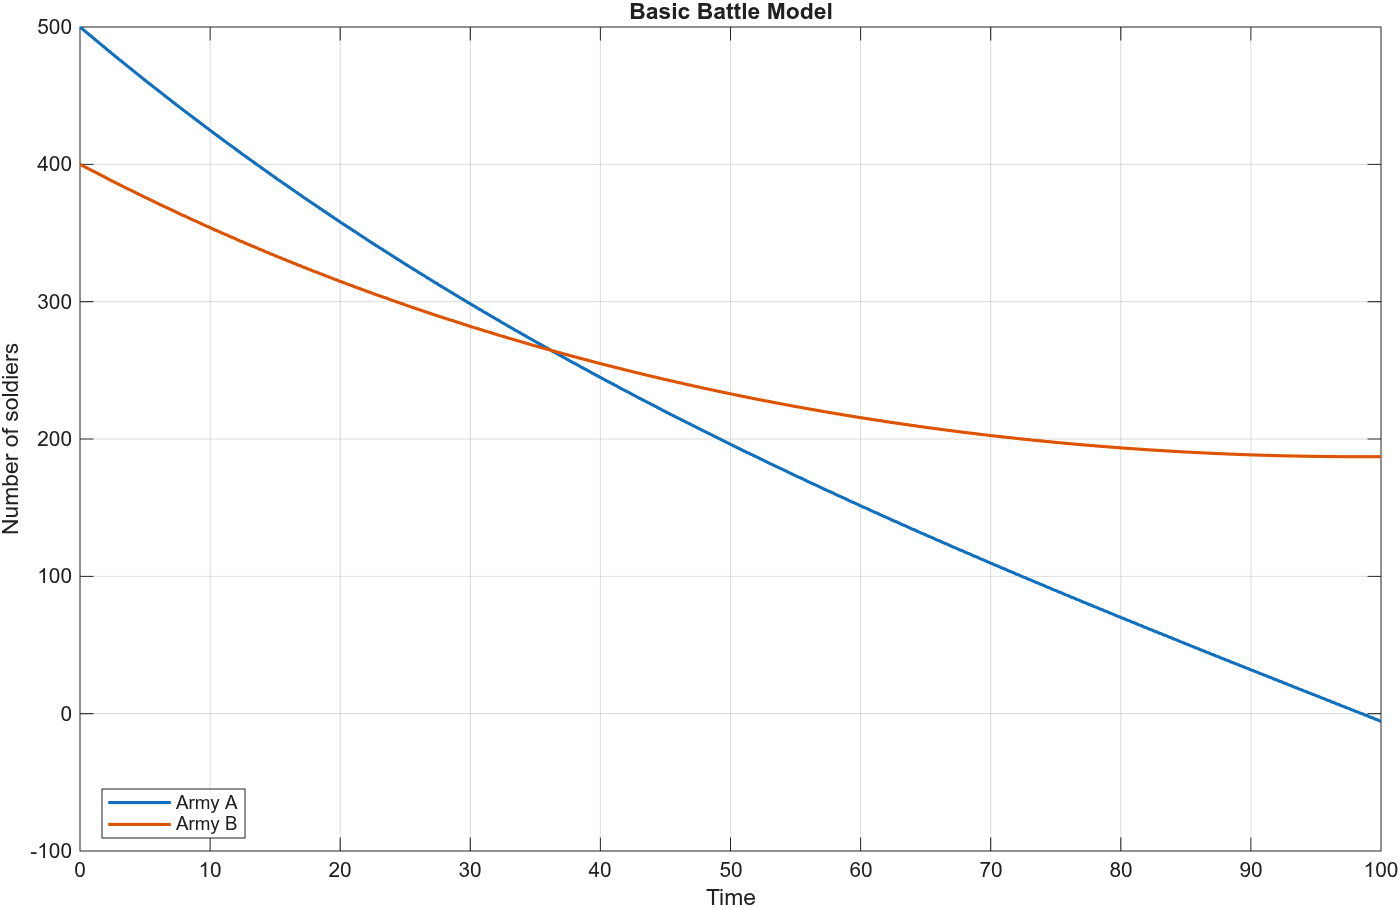
\includegraphics[width=0.7\textwidth]{Figure13.1.png}
\end{figure}

\vspace{1em}
\noindent
\textbf{Explanation of MATLAB commands}

\begin{enumerate}
    \item \textbf{a and b:} Store the fighting-effectiveness parameters.
    \item \textbf{x0 and y0:} Set the initial numbers of soldiers.
    \item \textbf{initial = [x0; y0]:} Stores the initial conditions in a column vector.
    \item \textbf{f = @(t,z) [...]:} Defines the two differential equations; $z(1)$ is Army A and $z(2)$ is Army B.
    \item \textbf{ode45:} Numerically solves the coupled differential equations.
    \item \textbf{Z(:,1), Z(:,2):} Extract the calculated strengths of the two armies.
    \item \textbf{plot and hold on:} Display both army strengths on the same graph.
    \item \textbf{legend:} Labels the curves; Location best lets MATLAB choose a suitable position.
\end{enumerate}

\vspace{1em}
\noindent
\textbf{Interpretation}
\begin{itemize}
    \item Both curves decrease because both armies lose soldiers.
    \item The slope indicates the rate at which an army is losing soldiers.
    \item The parameters $a$ and $b$ control the effectiveness of the opposing armies.
    \item The army whose strength reaches zero first is defeated in this simplified model. Interpret the solution only until a force is exhausted; negative soldier counts are not meaningful.
\end{itemize}

\vspace{1em}
\noindent
\textbf{\large{MATLAB Code (JUNGLE WARFARE MODEL):}}
\begin{lstlisting}
clc; clear; close all; 

% Model parameters 
a1 = 0.0001; a2 = 0.000001; 

% Initial army strengths
R0 = 1000; B0 = 1000; 

% Time interval 
tspan = [0 100]; 

% Initial conditions 
initial = [R0; B0]; 

% Jungle warfare model 
f = @(t,z) [-a1*z(2); -a2*z(1)*z(2)]; 

% Solve the differential equations
[t,Z] = ode45(f, tspan, initial); 

% Extract army strengths 
R = Z(:,1); B = Z(:,2); 

% Plot the results 
plot(t,R,'LineWidth',1.5); 
hold on; 
plot(t,B,'LineWidth',1.5); 
grid on; 
xlabel('Time'); 
ylabel('Number of soldiers'); 
title('Jungle Warfare Model'); 
legend('Red Army','Blue Army','Location','best'); 
hold off; 
\end{lstlisting}

\vspace{1em}
\noindent
\textbf{\large{Output (JUNGLE WARFARE MODEL):}}
\begin{figure}[htbp]
\centering
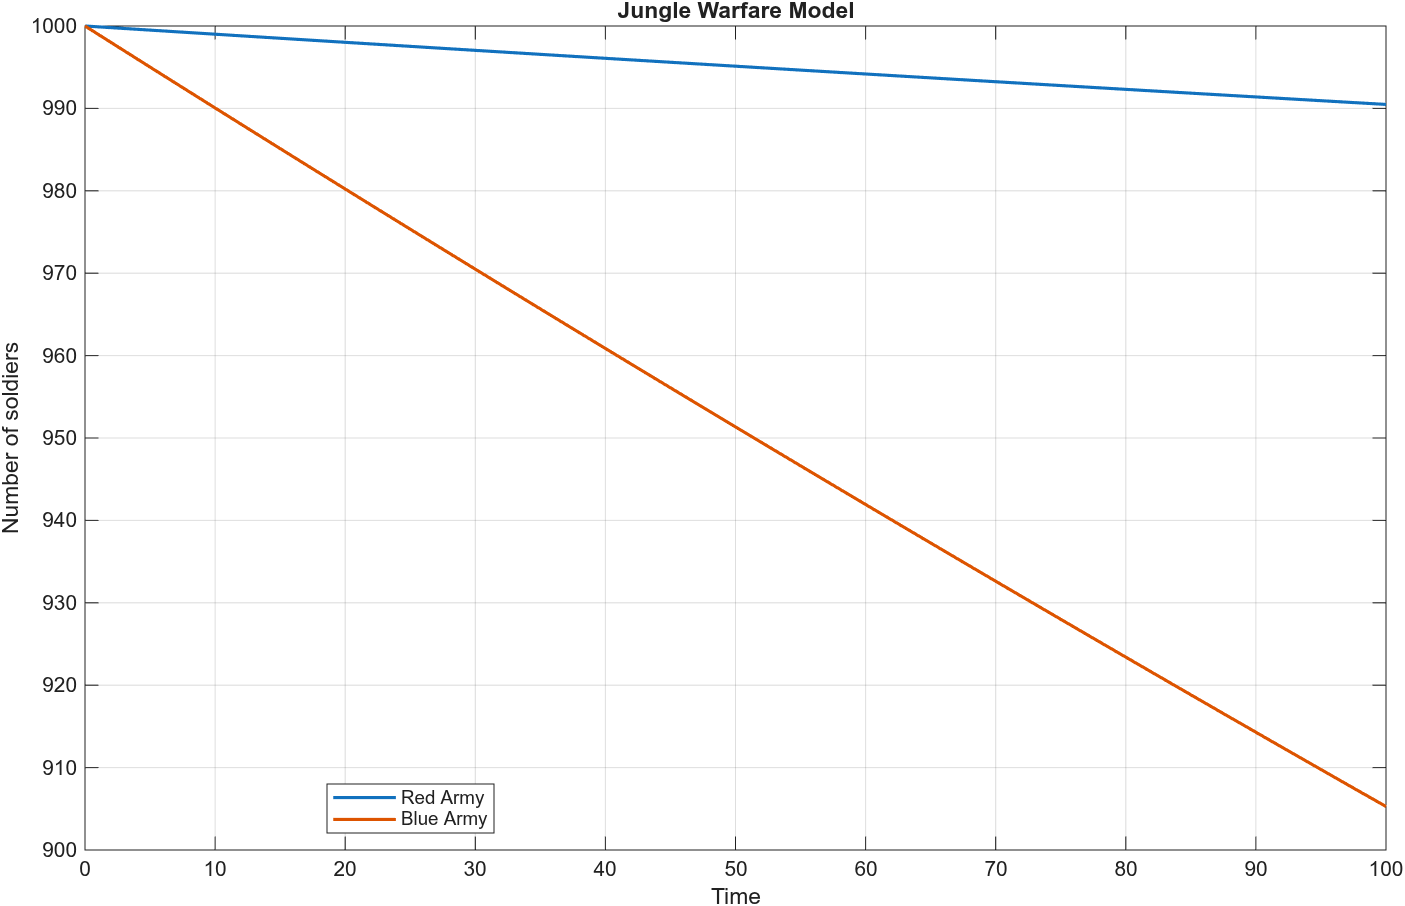
\includegraphics[width=0.7\textwidth]{Figure13.2.png}
\end{figure}

\vspace{1em}
\noindent
\textbf{Interpretation of the graph}
\begin{enumerate}
    \item Both army strengths decrease during the simulation because both derivatives are negative when populations and parameters are positive.
    \item The Red Army loss rate depends on $B$.
    \item The Blue Army loss rate depends on $R$ multiplied by $B$.
    \item Changing the parameters or initial populations changes the plotted curves.
\end{enumerate}

\end{document}
